\documentclass{article}\usepackage[]{graphicx}\usepackage[usenames,dvipsnames]{color}
%% maxwidth is the original width if it is less than linewidth
%% otherwise use linewidth (to make sure the graphics do not exceed the margin)
\makeatletter
\def\maxwidth{ %
  \ifdim\Gin@nat@width>\linewidth
    \linewidth
  \else
    \Gin@nat@width
  \fi
}
\makeatother

\definecolor{fgcolor}{rgb}{0.251, 0.251, 0.251}
\newcommand{\hlnum}[1]{\textcolor[rgb]{0.816,0.125,0.439}{#1}}%
\newcommand{\hlstr}[1]{\textcolor[rgb]{0.251,0.627,0.251}{#1}}%
\newcommand{\hlcom}[1]{\textcolor[rgb]{0.502,0.502,0.502}{\textit{#1}}}%
\newcommand{\hlopt}[1]{\textcolor[rgb]{0,0,0}{#1}}%
\newcommand{\hlstd}[1]{\textcolor[rgb]{0.251,0.251,0.251}{#1}}%
\newcommand{\hlkwa}[1]{\textcolor[rgb]{0.125,0.125,0.941}{#1}}%
\newcommand{\hlkwb}[1]{\textcolor[rgb]{0,0,0}{#1}}%
\newcommand{\hlkwc}[1]{\textcolor[rgb]{0.251,0.251,0.251}{#1}}%
\newcommand{\hlkwd}[1]{\textcolor[rgb]{0.878,0.439,0.125}{#1}}%
\let\hlipl\hlkwb

\newenvironment{knitrout}{}{} % an empty environment to be redefined in TeX
\usepackage{alltt}

\RequirePackage[]{/home/arvind/.R/x86_64-pc-linux-gnu-library/3.4/BiocStyle/resources/tex/Bioconductor2}
\AtBeginDocument{\bibliographystyle{/home/arvind/.R/x86_64-pc-linux-gnu-library/3.4/BiocStyle/resources/tex/unsrturl}}


\title{The Xeva User's Guide}
\author[1,2]{Arvind Mer}
\author[1,2,3]{Benjamin Haibe-Kains}
\affil[1]{Princess Margaret Cancer Centre, University Health Network, Toronto, Canada}
\affil[2]{Department of Medical Biophysics, University of Toronto, Toronto, Canada}
\affil[3]{Department of Computer Science, University of Toronto, Toronto, Canada}

\date{\today}
\IfFileExists{upquote.sty}{\usepackage{upquote}}{}
\begin{document}

\maketitle
\tableofcontents
\newpage



\section{Introduction}

The Xeva package provides efficient and powerful functions for patient-drived xenograft (PDX) based pharmacogenomic data analysis.

\section{Installation and Settings}

Xeva requires that several packages be installed. All dependencies are available from CRAN or Bioconductor:

\begin{knitrout}
\definecolor{shadecolor}{rgb}{0.941, 0.941, 0.941}\color{fgcolor}\begin{kframe}
\begin{alltt}
\hlkwd{source}\hlstd{(}\hlstr{'http://bioconductor.org/biocLite.R'}\hlstd{)}
\hlkwd{biocLite}\hlstd{(}\hlstr{'Xeva'}\hlstd{)}
\end{alltt}
\end{kframe}
\end{knitrout}

Load Xeva into your current workspace:
\begin{knitrout}
\definecolor{shadecolor}{rgb}{0.941, 0.941, 0.941}\color{fgcolor}\begin{kframe}
\begin{alltt}
\hlkwd{library}\hlstd{(Xeva)}
\end{alltt}
\end{kframe}
\end{knitrout}

Load the dataset you wish to analyze. For the sake of this tutorial, here we load the NIBR PDXE breast cancer dataset as an example:
\begin{knitrout}
\definecolor{shadecolor}{rgb}{0.941, 0.941, 0.941}\color{fgcolor}\begin{kframe}
\begin{alltt}
\hlkwd{data}\hlstd{(brca)}
\hlkwd{print}\hlstd{(brca)}
\end{alltt}
\begin{verbatim}
## Xeva-set name: PDXE.BRCA
## Creation date: Fri Sep 14 11:41:33 2018
## Number of models: 849
## Number of drugs: 22
## Moleculer dataset: RNASeq, mutation, cnv
\end{verbatim}
\end{kframe}
\end{knitrout}

\section{Definitions}
Before we further dive into the analysis and visualization, it is important to underastand the terminology used in the \Rpackage{Xeva} package.
In a \textbf{Xeva} object, the \textbf{experiment} slot stores the data for each individual PDX/mouse. With the exception of tumor growth data (time vs. tumor volume), for each individual PDX/mouse, you can access metadata such as the patient's age, sex, tissue histology, and passage information.
All of this metadata is stored in the \textbf{pdxModel} class, where a unique ID called \texttt{model.id} is given to each PDX/mouse model. As for the tumor growth information, Xeva provides separate functions for retrieving visualizing time vs. tumor volume data.
We will see later how to get these data for an individual \textit{model.id}, but first, let's define some other terms that appear in the \Rpackage{Xeva} package.

A PDX experiment can be one of the two categories:
\begin{itemize}
  \item \textbf{treatment} represents experiments in which the PDX receives some kind of drug (or drug combination)
  \item \textbf{control} represents experiments in which the PDX receives no drug
\end{itemize}

To see the effect of a drug, several replicate experiments are done for both the control and the treatment categories.
In \textbf{Xeva}, a collection of PDX \textit{model.ids} originating from the same patient is organized in \textbf{batches} (\textit{batch}). A \textit{batch} has two arms: \textit{control} and \textit{treatment}. This is illustrated in Figure~\ref{fig:1}.

\begin{figure}[!ht]
    \centering
    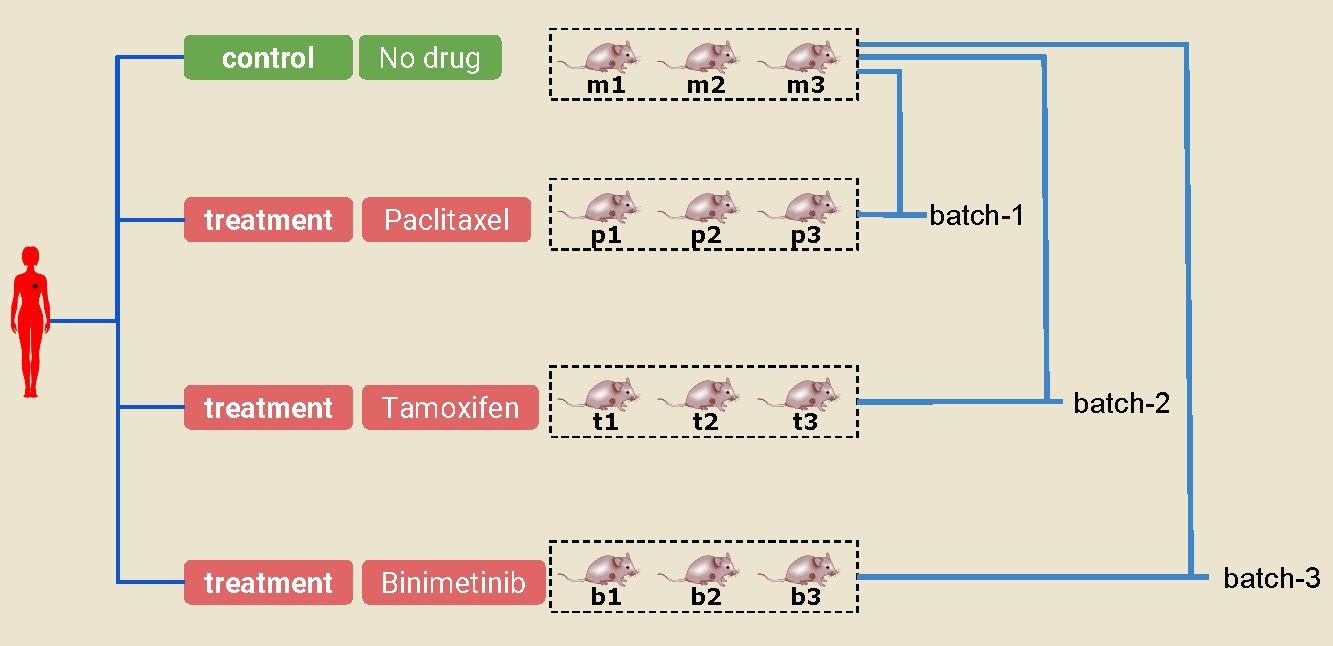
\includegraphics[keepaspectratio=true,width=1\textwidth]{images/Xeva_batch_2.pdf}
    \caption{A PDX experiment. The text under each of the PDX/mouse (ie. m1, m2, p1, etc.) denotes the \textit{model.id} in \textbf{Xeva}. In this example, three PDXs are delclared as control (m1, m2, and m3). Similarly, in the treatment arm, 3 PDXs are given the drug paclitaxel (p1, p2, and p3), 3 are given tamoxifen (t1, t2, and t3), and 3 are given binimetinib (b1, b2, b3). The PDXs in the control arm and one of the treatment arms together constitute a \textit{batch}. For example, control arm models (m1, m2, and m3) and treatment arm models (t1,t2, and t3) together create a batch called batch-2. } \label{fig:1}
\end{figure}

A \textbf{Xeva} object binds together all individual experiments, batch information, and molecular data into one single class called XevaSet.


\section{Data Access}
As mentioned earlier, \textbf{Xeva} stores metadata for each individual PDX model.
We can retrieve the meta-information about each PDX, such as number of models and tissue type, using:
\begin{knitrout}
\definecolor{shadecolor}{rgb}{0.941, 0.941, 0.941}\color{fgcolor}\begin{kframe}
\begin{alltt}
\hlstd{brca.mod} \hlkwb{<-} \hlkwd{modelInfo}\hlstd{(brca)}
\hlkwd{dim}\hlstd{(brca.mod)}
\end{alltt}
\begin{verbatim}
## [1] 849   5
\end{verbatim}
\begin{alltt}
\hlstd{brca.mod[}\hlnum{1}\hlopt{:}\hlnum{4}\hlstd{, ]}
\end{alltt}
\begin{verbatim}
##                model.id tissue   tissue.name patient.id        drug
## X.1004.BG98 X.1004.BG98   BRCA Breast Cancer     X-1004      BGJ398
## X.1004.biib X.1004.biib   BRCA Breast Cancer     X-1004 binimetinib
## X.1004.BK20 X.1004.BK20   BRCA Breast Cancer     X-1004      BKM120
## X.1004.BY19 X.1004.BY19   BRCA Breast Cancer     X-1004      BYL719
\end{verbatim}
\end{kframe}
\end{knitrout}
The output shows that the \textit{brca} dataset contains 849 PDX models.
We can also see the time vs. tumor volume data for a model using:

\begin{knitrout}
\definecolor{shadecolor}{rgb}{0.941, 0.941, 0.941}\color{fgcolor}\begin{kframe}
\begin{alltt}
\hlstd{model.data} \hlkwb{<-} \hlkwd{getExperiment}\hlstd{(brca,} \hlkwc{model.id} \hlstd{=} \hlstr{"X.1004.BG98"}\hlstd{)}
\hlkwd{head}\hlstd{(model.data)}
\end{alltt}
\begin{verbatim}
##      model.id drug.join.name time volume body.weight volume.normal
## 1 X.1004.BG98         BGJ398    0  199.7        28.2     0.0000000
## 2 X.1004.BG98         BGJ398    2  181.9        28.0    -0.0891337
## 3 X.1004.BG98         BGJ398    5  172.7        28.4    -0.1352028
## 4 X.1004.BG98         BGJ398    9  129.6        27.2    -0.3510265
## 5 X.1004.BG98         BGJ398   12   91.3        26.7    -0.5428142
## 6 X.1004.BG98         BGJ398   16  117.1        26.2    -0.4136204
\end{verbatim}
\end{kframe}
\end{knitrout}

Similarly, for \textbf{batch} names, we can obtain all predefined batch names using:

\begin{knitrout}
\definecolor{shadecolor}{rgb}{0.941, 0.941, 0.941}\color{fgcolor}\begin{kframe}
\begin{alltt}
\hlstd{batch.name} \hlkwb{<-} \hlkwd{batchInfo}\hlstd{(brca)}
\hlstd{batch.name[}\hlnum{1}\hlopt{:}\hlnum{4}\hlstd{]}
\end{alltt}
\begin{verbatim}
## [1] "X-1004.BGJ398"      "X-1004.binimetinib" "X-1004.BKM120"     
## [4] "X-1004.BYL719"
\end{verbatim}
\end{kframe}
\end{knitrout}

The information about a \textbf{batch} can be shown using:
\begin{knitrout}
\definecolor{shadecolor}{rgb}{0.941, 0.941, 0.941}\color{fgcolor}\begin{kframe}
\begin{alltt}
\hlkwd{batchInfo}\hlstd{(brca,} \hlkwc{batch} \hlstd{=} \hlstr{"X-1004.binimetinib"}\hlstd{)}
\end{alltt}
\begin{verbatim}
## $`X-1004.binimetinib`
## name = X-1004.binimetinib
## control = X.1004.uned
## treatment = X.1004.biib
\end{verbatim}
\end{kframe}
\end{knitrout}
Here, for the batch named \textit{X-1004.binimetinib}, we can see that the control sample is \textit{X.1004.uned} and the treatment sample is \textit{X.1004.biib}.



\section{Visualizing PDX Growth Curve}

Xeva provides a function to plot time vs. tumor volume data for individual models as well as for individual batches. These data can be plotted by using the name of the batch:
\begin{knitrout}
\definecolor{shadecolor}{rgb}{0.941, 0.941, 0.941}\color{fgcolor}\begin{kframe}
\begin{alltt}
\hlkwd{plotPDX}\hlstd{(brca,} \hlkwc{batch} \hlstd{=} \hlstr{"X-4567.BKM120"}\hlstd{)}
\end{alltt}
\end{kframe}\begin{figure*}
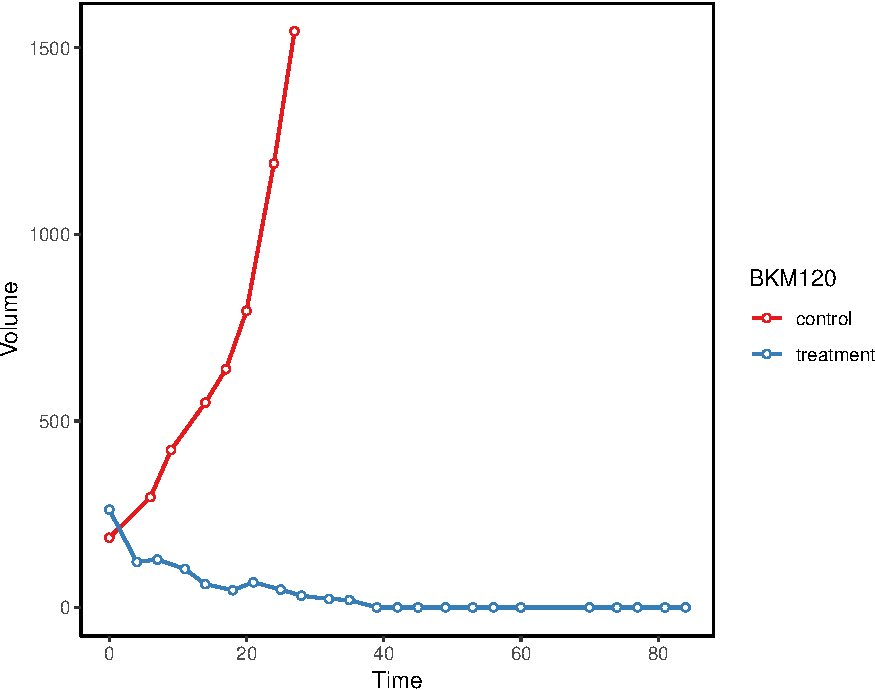
\includegraphics[width=4in]{figure/plot1-1} \caption{Tumor growth curve for a batch of control and treated PDXs}\label{fig:plot1}
\end{figure*}

\end{knitrout}


You can choose to see different aspects of this visualization. For example, we can plot normalized volume; we can also change the colors of the lines:
\begin{knitrout}
\definecolor{shadecolor}{rgb}{0.941, 0.941, 0.941}\color{fgcolor}\begin{kframe}
\begin{alltt}
\hlkwd{plotPDX}\hlstd{(brca,} \hlkwc{batch} \hlstd{=} \hlstr{"X-4567.BKM120"}\hlstd{,} \hlkwc{vol.normal} \hlstd{= T,} \hlkwc{control.col} \hlstd{=} \hlstr{"#a6611a"}\hlstd{,}
        \hlkwc{treatment.col} \hlstd{=} \hlstr{"#018571"}\hlstd{,} \hlkwc{major.line.size} \hlstd{=} \hlnum{1}\hlstd{,} \hlkwc{max.time} \hlstd{=} \hlnum{40}\hlstd{)}
\end{alltt}
\end{kframe}\begin{figure*}
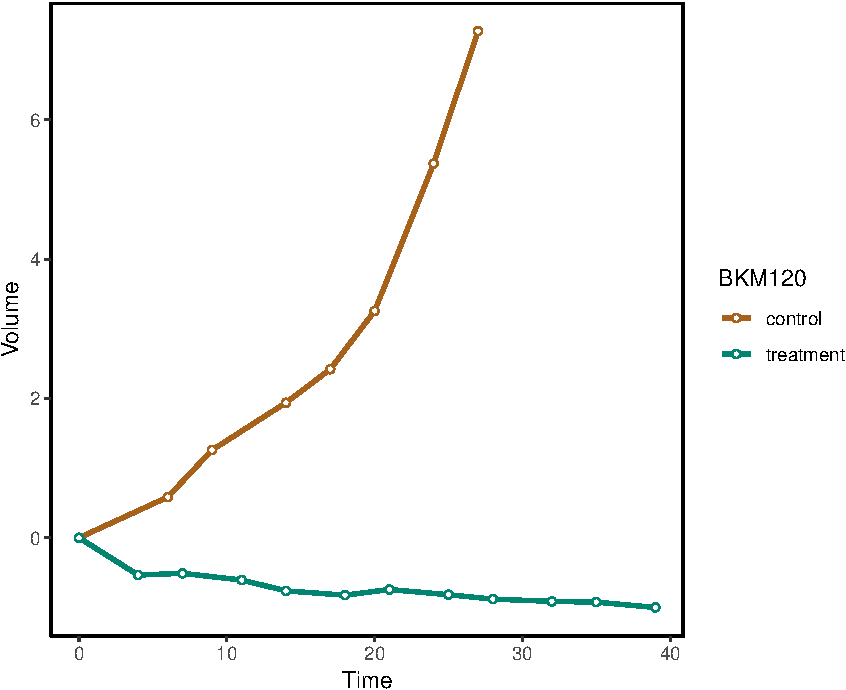
\includegraphics[width=4in]{figure/pdxplot2-1} \caption{Tumor growth curve for a batch of control and treated PDX. Here, the volume is normalized and plots are truncated at 40 days}\label{fig:pdxplot2}
\end{figure*}

\end{knitrout}


Data can also be visualized at the patient level by specifying \texttt{patient.id}:
%%##X-2344, X-1004, X-3078 and X-5975
\begin{knitrout}
\definecolor{shadecolor}{rgb}{0.941, 0.941, 0.941}\color{fgcolor}\begin{kframe}
\begin{alltt}
\hlkwd{plotPDX}\hlstd{(brca,} \hlkwc{patient.id}\hlstd{=}\hlstr{"X-3078"}\hlstd{,} \hlkwc{drug}\hlstd{=}\hlstr{"paclitaxel"}\hlstd{,}\hlkwc{control.name} \hlstd{=} \hlstr{"untreated"}\hlstd{)}
\end{alltt}
\end{kframe}\begin{figure*}
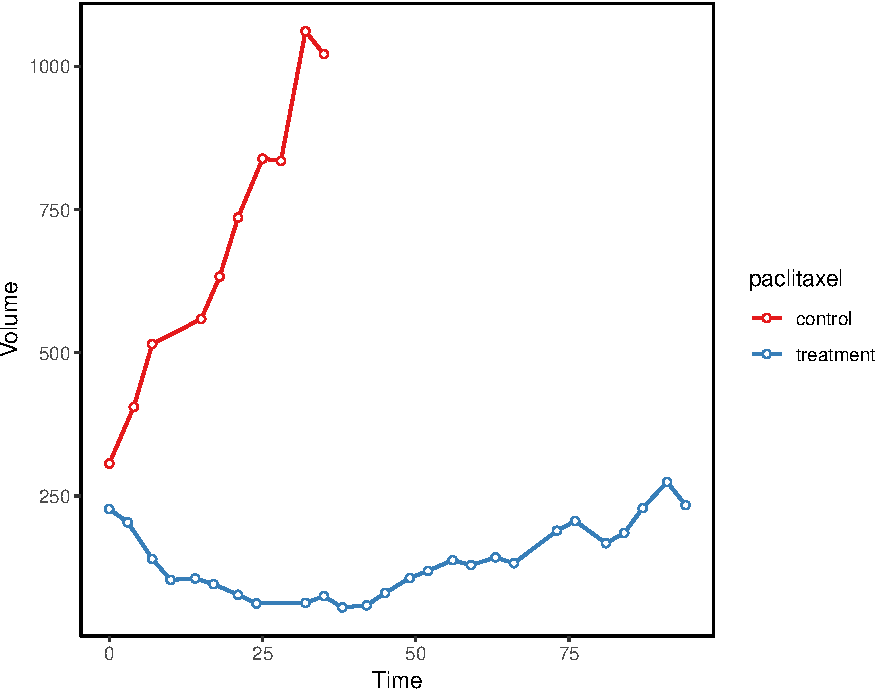
\includegraphics[width=4in]{figure/pdxplot3-1} \caption{Tumor growth curve for a batch of control and treated PDX generated using patient ID and drug name}\label{fig:pdxplot3}
\end{figure*}

\end{knitrout}


\section{PDX Model Response}
Xeva can effectively summarize PDX drug response data. Here we summarize the \textbf{mRECIST} values for the models in our dataset:

\begin{knitrout}
\definecolor{shadecolor}{rgb}{0.941, 0.941, 0.941}\color{fgcolor}\begin{kframe}
\begin{alltt}
\hlstd{brca.mr} \hlkwb{<-} \hlkwd{summarizeResponse}\hlstd{(brca,} \hlkwc{response.measure} \hlstd{=} \hlstr{"mRECIST"}\hlstd{)}
\hlstd{brca.mr[}\hlnum{1}\hlopt{:}\hlnum{5}\hlstd{,} \hlnum{1}\hlopt{:}\hlnum{4}\hlstd{]}
\end{alltt}
\begin{verbatim}
##                 X-1004 X-1008 X-1286 X-1298
## BGJ398              PR     SD     PD     SD
## binimetinib         PD     SD     SD     PD
## BKM120              SD     SD     SD     PR
## BYL719              SD     PR     SD     PD
## BYL719 + LEE011     PD     SD     SD     PD
\end{verbatim}
\end{kframe}
\end{knitrout}

These \textbf{mRECIST} values can be visualized using:
\begin{knitrout}
\definecolor{shadecolor}{rgb}{0.941, 0.941, 0.941}\color{fgcolor}\begin{kframe}
\begin{alltt}
\hlkwd{plotmRECIST}\hlstd{(brca.mr,} \hlkwc{control.name}\hlstd{=}\hlstr{"untreated"}\hlstd{,} \hlkwc{row_fontsize}\hlstd{=}\hlnum{13}\hlstd{,} \hlkwc{col_fontsize}\hlstd{=}\hlnum{12}\hlstd{)}
\end{alltt}
\end{kframe}\begin{figure*}
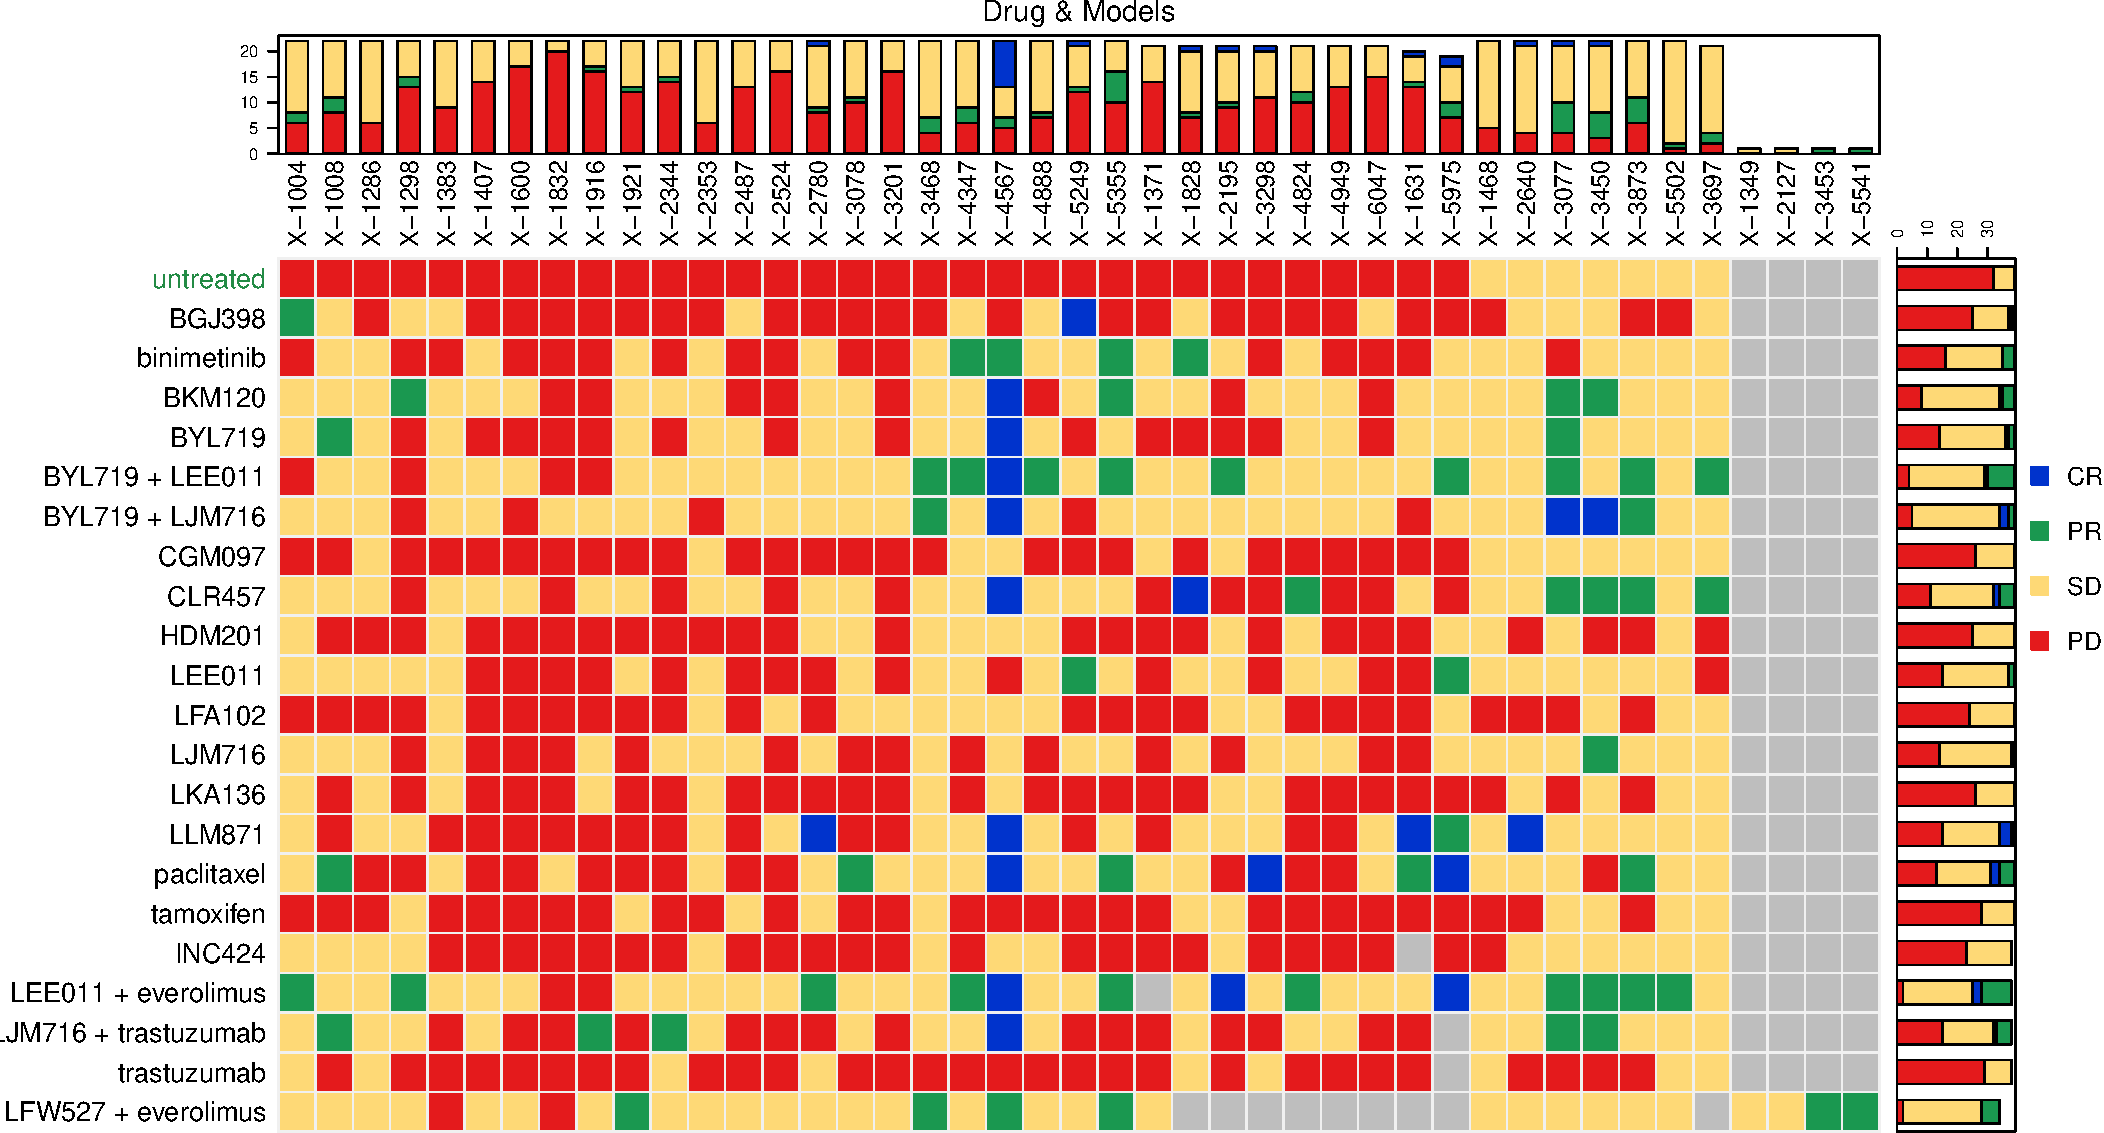
\includegraphics[width=\maxwidth]{figure/mR_BRCA-1} \caption{mRECIST plot for PDXE breast cancer data}\label{fig:mR_BRCA}
\end{figure*}

\end{knitrout}


Waterfall plots are also commonly used to visualize PDX drug response data.
Xeva provides a function to visualize and color waterfall plots:
\begin{knitrout}
\definecolor{shadecolor}{rgb}{0.941, 0.941, 0.941}\color{fgcolor}\begin{kframe}
\begin{alltt}
\hlkwd{waterfall}\hlstd{(brca,} \hlkwc{drug}\hlstd{=}\hlstr{"binimetinib"}\hlstd{,} \hlkwc{res.measure}\hlstd{=}\hlstr{"best.average.response"}\hlstd{)}
\end{alltt}
\end{kframe}\begin{figure*}
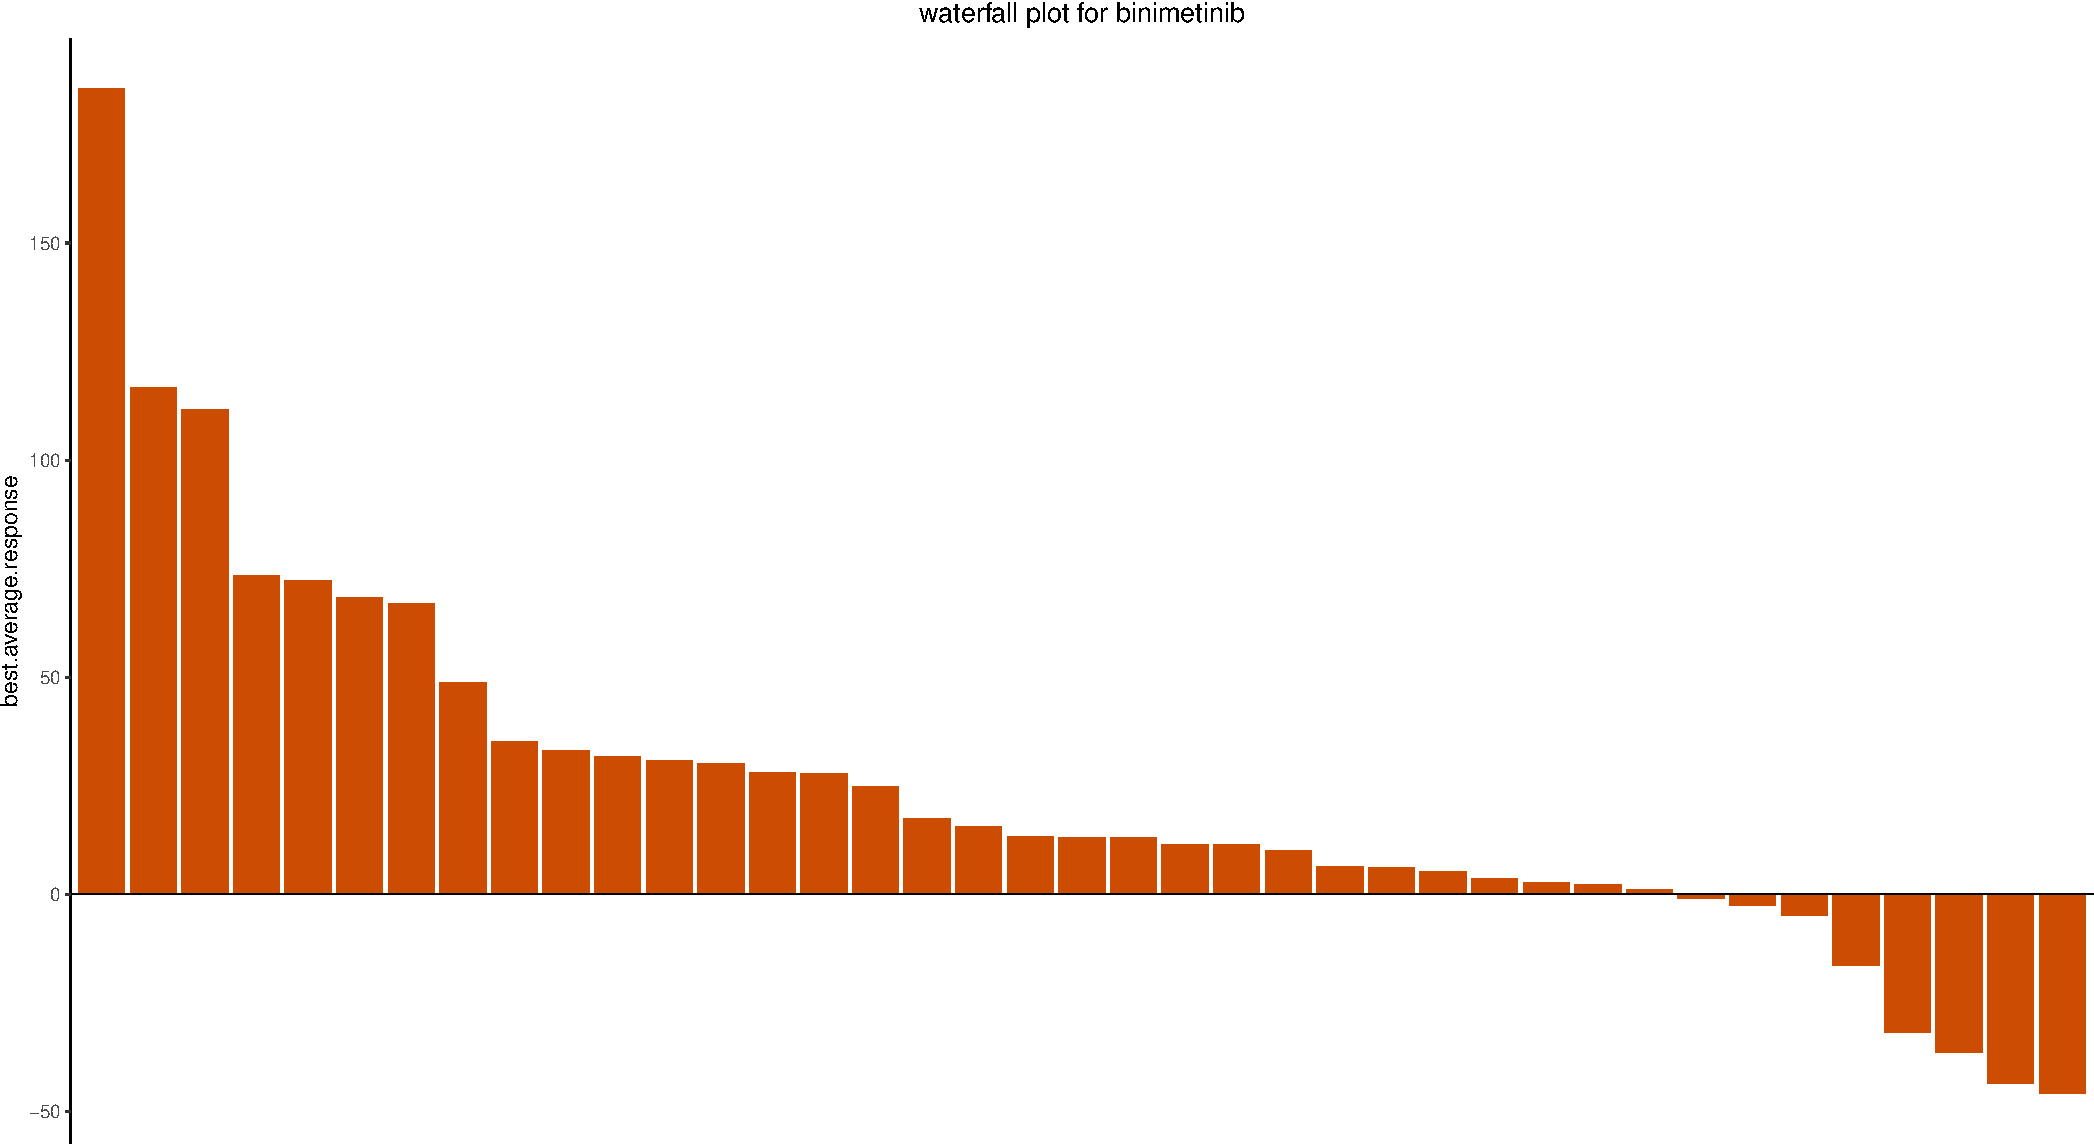
\includegraphics[width=\maxwidth]{figure/waterFall1-1} \caption{Waterfall plot for binimetinib drug response in PDXs}\label{fig:waterFall1}
\end{figure*}

\end{knitrout}


It is useful to color the bars of your waterfall plot by genomic properties.
Here we create a waterfall plot for drug BYL719 and color it based on the mutation status of the CDK13 gene.
First, we extract the genomic data for the models. Then, we can plot the waterfall plots:
\begin{knitrout}
\definecolor{shadecolor}{rgb}{0.941, 0.941, 0.941}\color{fgcolor}\begin{kframe}
\begin{alltt}
\hlstd{mut} \hlkwb{<-} \hlkwd{summarizeMolecularProfiles}\hlstd{(brca,}\hlkwc{drug} \hlstd{=} \hlstr{"BYL719"}\hlstd{,} \hlkwc{mDataType}\hlstd{=}\hlstr{"mutation"}\hlstd{)}
\end{alltt}


{\ttfamily\noindent\itshape\color{messagecolor}{\#\# Loading required package: Biobase}}

{\ttfamily\noindent\itshape\color{messagecolor}{\#\# Loading required package: BiocGenerics}}

{\ttfamily\noindent\itshape\color{messagecolor}{\#\# Loading required package: parallel}}

{\ttfamily\noindent\itshape\color{messagecolor}{\#\# \\\#\# Attaching package: 'BiocGenerics'}}

{\ttfamily\noindent\itshape\color{messagecolor}{\#\# The following objects are masked from 'package:parallel':\\\#\# \\\#\#\ \ \ \  clusterApply, clusterApplyLB, clusterCall, clusterEvalQ,\\\#\#\ \ \ \  clusterExport, clusterMap, parApply, parCapply, parLapply,\\\#\#\ \ \ \  parLapplyLB, parRapply, parSapply, parSapplyLB}}

{\ttfamily\noindent\itshape\color{messagecolor}{\#\# The following objects are masked from 'package:stats':\\\#\# \\\#\#\ \ \ \  IQR, mad, sd, var, xtabs}}

{\ttfamily\noindent\itshape\color{messagecolor}{\#\# The following objects are masked from 'package:base':\\\#\# \\\#\#\ \ \ \  anyDuplicated, append, as.data.frame, cbind, colMeans, colnames,\\\#\#\ \ \ \  colSums, do.call, duplicated, eval, evalq, Filter, Find, get,\\\#\#\ \ \ \  grep, grepl, intersect, is.unsorted, lapply, lengths, Map,\\\#\#\ \ \ \  mapply, match, mget, order, paste, pmax, pmax.int, pmin,\\\#\#\ \ \ \  pmin.int, Position, rank, rbind, Reduce, rowMeans, rownames,\\\#\#\ \ \ \  rowSums, sapply, setdiff, sort, table, tapply, union, unique,\\\#\#\ \ \ \  unsplit, which, which.max, which.min}}

{\ttfamily\noindent\itshape\color{messagecolor}{\#\# Welcome to Bioconductor\\\#\# \\\#\#\ \ \ \  Vignettes contain introductory material; view with\\\#\#\ \ \ \  'browseVignettes()'. To cite Bioconductor, see\\\#\#\ \ \ \  'citation("{}Biobase"{})', and for packages 'citation("{}pkgname"{})'.}}\begin{alltt}
\hlstd{model.type} \hlkwb{<-} \hlstd{Biobase}\hlopt{::}\hlkwd{exprs}\hlstd{(mut)[}\hlstr{"CDK13"}\hlstd{, ]}
\hlstd{model.type[}\hlkwd{grepl}\hlstd{(}\hlstr{"Mut"}\hlstd{, model.type)]} \hlkwb{<-} \hlstr{"mutation"}
\hlstd{model.type[model.type}\hlopt{!=}\hlstr{"mutation"}\hlstd{]} \hlkwb{<-} \hlstr{"wild type"}
\hlstd{model.color} \hlkwb{<-} \hlkwd{list}\hlstd{(}\hlstr{"mutation"}\hlstd{=}\hlstr{"#fb8072"}\hlstd{,} \hlstr{"wild type"}\hlstd{=}\hlstr{"#80b1d3"}\hlstd{)}
\hlkwd{waterfall}\hlstd{(brca,} \hlkwc{drug}\hlstd{=}\hlstr{"BYL719"}\hlstd{,} \hlkwc{res.measure}\hlstd{=}\hlstr{"best.average.response"}\hlstd{,}
          \hlkwc{model.id}\hlstd{=}\hlkwd{names}\hlstd{(model.type),} \hlkwc{model.type}\hlstd{= model.type,}
          \hlkwc{type.color} \hlstd{= model.color)}
\end{alltt}
\end{kframe}\begin{figure*}
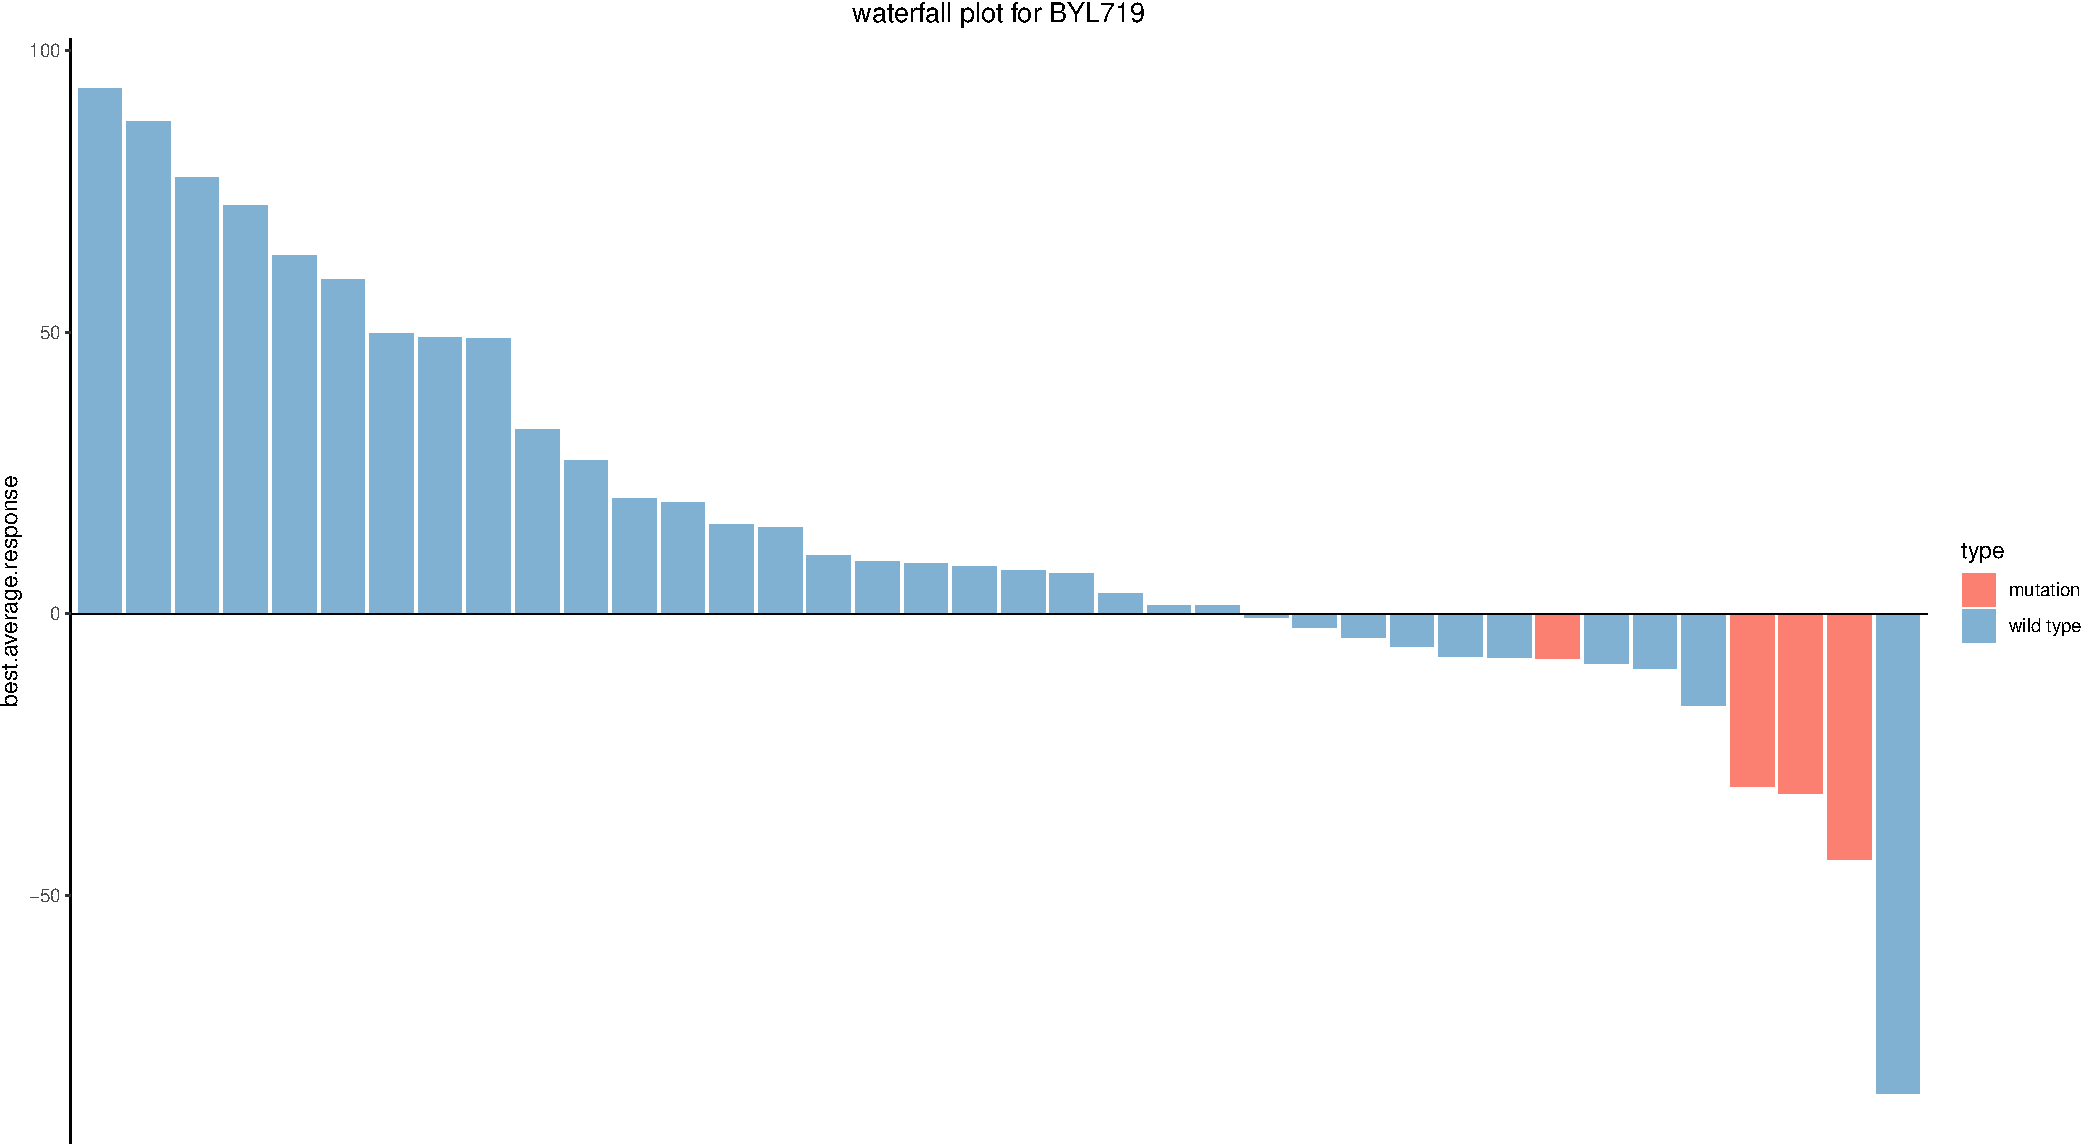
\includegraphics[width=\maxwidth]{figure/waterFall2-1} \caption{Waterfall plot for binimetinib drug response in PDXs}\label{fig:waterFall2}
\end{figure*}

\end{knitrout}


\end{document}
